% Example article for the KIO journal

\documentclass[eqsecnum,authorsinfo]{kioj6}


% You can load your own packages here.
\usepackage{enumitem}
\usepackage{tabularray}


% ========== BIBLIOGRAPHY APPEARANCE ==========
%
% \newcommand{\bibfontsize}{\footnotesize}   % bibliography font size
% \newcommand{\biblinespread}{1.1}           % line spacing within an entry
% \newcommand{\bibitemsep}{0pt}              % vertical gap between entries


% ========== SETTINGS TO PREVENT WIDOW LINES ==========
%\raggedbottom
%\widowpenalty=10000
%\clubpenalty=10000

% ===================== JOURNAL SETTINGS ====================

% Page number on which the article starts
\setcounter{page}{2}

% Journal section (may not be known at submission time)

%\journalsectionnoimage{algorithmic-mathematics}
%\journalsectionnoimage{artificial-intelligence}
%\journalsectionnoimage{informatics}
%\journalsectionnoimage{information-systems}
%\journalsectionnoimage{software-engineering}
%\journalsectionnoimage{computer-in-education}
%\journalsectionnoimage{popular-science-articles}
%\journalsectionnoimage{programming-practice}
%\journalsectionnoimage{editorial-column}
%\journalsectionnoimage{specialists-training-new-teaching-methods}
%\journalsectionnoimage{specialists-training-training-programs}
%\journalsectionnoimage{specialists-training-professional-standards}
%\journalsectionnoimage{open-problems-for-young-scientists}
\journalsectionnoimage{empty}

% Year is set; the issue number is unknown so a dash is used.
% "edu" stands for the "Computer Tools in Education" journal.

\issue{2026}{1}{edu}

% ===== ARTICLE TYPE ====

% 1. {1}  -> Research article
% 2. {2}  -> Review article
% 3. {3}  -> Conference paper
% 4. {4}  -> Editorial article
% 5. {5}  -> Discussion article
% 6. {6}  -> Short Communication
%
% =========================

\articletype{1}


\udknumber{999.999}
\doinumber{10.32603/2071-2340-2026-2-XXX-XXX}

% =============== RUSSIAN-LANGUAGE DATA ===============

% Article title (Russian)
\title[К вопросу об оформлении научных статей]{К вопросу об оформлении научных статей с~использованием современных технических средств на~основе пакета прикладного ПО \LaTeX}

% Authors (Russian version)
\author{1}[Андреев А.~А.\affil{1,3}]{Андреев Аркадий Александрович}
\authorinfo{1}{доктор физ.-мат. наук, профессор кафедры алгоритмической математики, СПбГЭТУ «ЛЭТИ»}
\authororcid{1}{orcid.org/0000-0000-9999-9999}
\authoremailEnvelope{1}{aaandreev@etu.ru} % адрес для корреспонденции

\author{2}[Богоявленский М. М.\affil{2}]{Богоявленский Максим Маратович}
\authorinfo{2}{канд. физ.-мат. наук, старший нучный сотрудник Лаборатории радиоастрономических наблюдений ИПА РАН}
\authoremail{2}{mmb@iaaras.ru}

\author{3}[Воронов В.~В.\affil{3}]{Воронов Владимир Владимирович}
\authorinfo{3}{аспирант, ассистент факультета математики и компьютерных наук СПбГУ}
\authoremail{3}{v.v.voronov@spbu.ru}

\author{4}[Ге В.~Г.\affil{4}]{Ге Вильгельмина Геннадьевна}
\authorinfo{4}{руководитель отдела контроля качества компании «Квантори»}
\authororcid{4}{orcid.org/0000-9999-9999-9999}
\authoremail{4}{vilgelmina.g.ge@quantori.com}


% Affiliations
\affiliation{1}{Санкт-Петербургский государственный электротехнический университет «ЛЭТИ» им. В. И. Ульянова (Ленина), Российская Федерация, 197022, Санкт-Петербург,
ул. Профессора Попова, 5}
\affiliation{2}{Институт прикладной астрономии Российской академии наук, Российская Федерация, 191187, Санкт-Петербург, наб. Кутузова, 10}
\affiliation{3}{Санкт-Петербургский государственный университет, Российская Федерация, 199034, Санкт-Петербург, Университетская наб., 7–9}
\affiliation{4}{Компания «Квантори», 1 Бродвей, Кембридж, Массачусетс, 02142, Соединенные Штаты}

% ========== ENGLISH-LANGUAGE DATA ==========

% Article title (English)
\titleen[On Typography of Scientific Articles]{On Typography of Scientific Articles Using Modern Tools Based on Software from the \LaTeX\ Family}

% Authors (English version)
\authoren{1}[Andreev A.~A.\affil{1,2}]{Andreev Arkady}
\authorinfoen{1}{ Dr. Sci. (Phys.-Math.), Professor at the Department of Algorithmic Mathematics, ETU ``LETI''}

\authoren{2}[Bogoyavlenskiy M.~M.\affil{2}]{Bogoyavlenskiy Maksim}
\authorinfoen{2}{Cand. Sci. (Phys.-Math.), Senior Researcher at the Laboratory of Radioastronomical Observations, IAA RAS}

\authoren{3}[Voronov V.~V.\affil{3}]{Voronov Vladimir}
\authorinfoen{3}{postgraduate, assistance lecturer at the Faculty of Mathematics and Computer Science, SPbSU}

\authoren{4}[Ge V.~G.\affil{4}]{Ge Vilgelmina}
\authorinfoen{4}{Head of Quality Assurance, Quantori LLC}


% Affiliations (English)
\affiliationen{1}{Saint Petersburg State Electrotechnical University “LETI”, Professora Popova ul. 5, St. Petersburg, 197022, Russian Federation}
\affiliationen{2}{Institute of Applied Astronomy of the Russian Academy of Sciences, Kutuzova nab. 10, \\ St. Petersburg, 191187, Russian Federation}
\affiliationen{3}{Saint Petersburg State University, Universitetskaya nab. 7–9, St. Petersburg, 199034, Russian Federation}
\affiliationen{4}{Quantori LLC, 1 Broadway, Cambridge, MA 02142, United States}

\begin{document}

	% ========== ENGLISH MAIN PART ==========

	\englishversion

	\maketitle

	\pagestyle{mainstyle}

	\begin{abstract}
		English abstract goes here.
		\keywordsen{keyword1, keyword2, keyword3}

		\autocitation
        %Or manual citation: \manualcitation{text}
	\end{abstract}

    \section{Introduction}
    The journal ``Computer Tools in Education'' has been published since January 1998.

    The scientific scope of the periodical is: algorithmic mathematics and mathematical modelling, computer science and information technology, automation of processes in education.

    Historically the journal has formed a common space for discussing problems related to enriching mathematics and computer science education through the use of computer tools.
    Because the use of computer tools today directly influences mathematics itself, the journal pays more and more attention to computer mathematics and computer science.
    The journal also focuses on bringing current research to students, so it welcomes papers that explain new ideas in computer science and algorithmic mathematics, as well as papers that pose problems for young researchers.

    \section{Formatting examples}\label{sec:formatting}
    Section headers are rendered in uppercase. There is no need to upper-case them in the source file.
    That way, the section name will remain in normal case in PDF table of contents.

    Now an example of a numbered list. Please pay attention to punctuation.
    \begin{enumerate}
        \item First item;
        \item Second item;
        \item Third item.
    \end{enumerate}

    \subsection{Figures}

    
    Fig.~\ref{fig:example} is a normal raster image with a caption.

    \begin{figure}[htb]
        \centering
        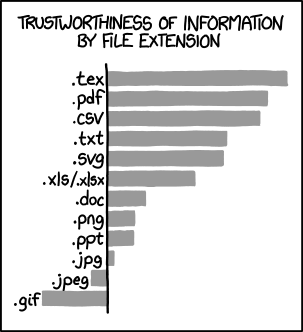
\includegraphics[width=0.4\textwidth]{xkcd1301.png}
        \caption{Reliability of information depending on the file extension} \label{fig:example}
    \end{figure}

    \subsubsection{Composite figures}

    Fig.~\ref{fig:example-2} contains two vector images: \ref{fig:example-2a} и \ref{fig:example-2b}.
    
    \begin{figure}[H]
        \centering
        \begin{subfigure}[t]{70mm}
             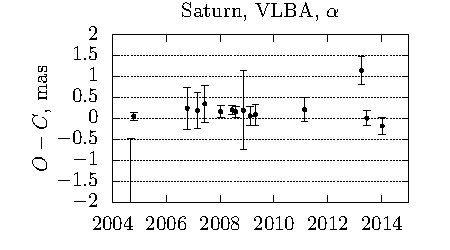
\includegraphics{saturn-vlba-alpha.pdf}
         \subcaption{Optional caption}
         \label{fig:example-2a}
        \end{subfigure}
        \ %space between images
        \begin{subfigure}[t]{70mm}
         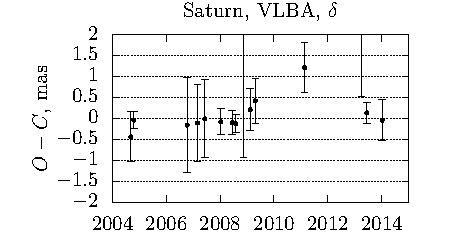
\includegraphics{saturn-vlba-delta.pdf}
            \subcaption{} % Здесь подзаголовок не указан
            \label{fig:example-2b}
        \end{subfigure}
        \caption{Two subfigures side by side} \label{fig:example-2}
    \end{figure}

    \subsection{Tables}

    \subsubsection{\texttt{tabular}}
\begin{table}[ht]
  \centering
\caption{G3-G5 solar storms in 2024 with their respective dates of forecase and dates and times of shock wave arrival}
\label{tbl:events}
\begin{tabular}{|c|c|c|} \hline
  Dst ranging,   & Date     & Shock wave            \\
  G-scale               & of forecast &  arrival time \\ \hline
  \#1 (G5) & 2024-05-10 & 2024-05-11T11  \\ \hline
  \#2 (G5) & 2024-05-09 & 2024-05-10T17  \\ \hline 
  \#3,4 (G4--3) & 2024-10-09 & 2024-10-11T15  \\ \hline 
  \#6 (G3) & 2024-05-10 & 2024-05-12T10  \\ \hline 
  \#5,9 (G4) & 2024-08-10    & 2024-08-11T07  \\ \hline
  \#7 (G3) & 2024-10-06 & 2024-10-06T08  \\ \hline 
  \#8 (G4) & 2024-03-23 & 2024-03-24T15 \\ \hline
  \#10 (G3) & 2024-04-18 & 2024-04-19T06 \\ \hline
  \#11 (G4) & 2024-09-14 & 2024-09-16T23\\ \hline
  \#12 (G3) & 2024-08-01 & 2024-08-04T15 \\ \hline
  \#13 (G3) & 2024-09-10 & 2024-09-12T04\\ \hline
  \#15 (G4) & 2024-06-25 & 2024-06-28T11\\ \hline 
\end{tabular}
\end{table}
    
    
    \subsubsection{\texttt{tblr}}
    \begin{table}[H]
  \centering
  \caption{Complex table}
  \label{tbl:complex}      
\begin{tblr}{
  hlines, vlines, % borders around each cell
  rowsep=0pt, colsep = 0pt,
  rows = {20pt}, columns = {100pt}, % fixed width columns and fixed height rows
  cells = {c,m}, % centered cells (vertically and horizontally)
  cell{1}{1} = {r=2}{}, % multirow
  cell{1}{2} = {c=2}{}, % multicolumn
}
State of Health & Fasting Value &         & After Eating         \\
                & Minimum       & Maximum & 2 hours after eating \\
Healthy         & 70            & 100     & Less than 140        \\
Pre-Diabetes    & 101           & 126     & 140 to 200           \\
Diabetes        & More than 126 & N/A     & More than 200        \\
\end{tblr}
\end{table}

    \subsection{Equations}

    Eq.~(\ref{eq:gaussian}) is numbered because it is references to.
    
    \begin{equation}
        \int_{-\infty}^{\infty} e^{-x^2} \, \mathrm{d}x = \sqrt{\pi}
        \label{eq:gaussian}
    \end{equation}
    
    Displayed equations can be unnumbered as well, for instance:

    $$\frac{d}{dt} \left( \frac{\partial L}{\partial \dot{\symbfit{q}}} \right) = \frac{\partial L}{\partial \symbfit{q}},$$

    \noindent where $L$ is the Lagrangian, $\symbfit{q}$ are generalized coordinates, and $\dot{\symbfit{q}}$
    are generalized velocities.
    
    \section{Reference examples}
    Reference to Sec.~\ref{sec:formatting}.

    Below you can find references for all kinds of bibliographical sources. You can
    use their Bibtex entries as templates for your own bibliography.

    About half of bibliography entries used in this text are stored in  \texttt{references-en.bib}.
    The other half are stored in \texttt{references.bib}. There is no need to use two files,
    it is normal to have only one for English manuscripts (Russian manuscripts are another story.)
    
    \begin{enumerate}
        \item \textbf{Books and chapters}
        \begin{itemize}[nosep]
            \item English-language book~---~\cite{Hairer}.
            \item Russian-language book without an author's English title translation~---~\cite{Gubanov}.
            \item Chapter in a Russian-language book~---~\cite{layexpl7}.
            \item Book chapter with edition, chapter, section and page range~---~\cite{ogura}.
            \item Multi-author book with several editors~---~\cite{HastieTibshiraniFriedman2009}.
            \item Chapter with several authors, editor and edition~---~\cite{Alberts2014CellCycle}.
            \item Chapter written by the volume editor~---~\cite{Gowers2008LanguageGrammar}.
            \item Chapter with a translator~---~\cite{Aleksandrov1963GeneralView}.
        \end{itemize}

        \item \textbf{Articles}
        \begin{itemize}[nosep]
            \item Russian-language article with an author's English title translation~---~\cite{Matveenko}.
            \item Periodical with article ID (Art.~no.)~---~\cite{Abbott2016GW150914}.
        \end{itemize}

        \item \textbf{Blog}~---~\cite{Dmitry2024Python}

        \item \textbf{Conference paper presented at a conference (no proceedings)}~---~\cite{Caratelli}.

        \item \textbf{Conference proceedings paper}~---~\cite{BYSIS2022}

        \item \textbf{Online dataset}~---~\cite{pavlov_2025_14923680}

        \item \textbf{Manual}
        \begin{itemize}[nosep]
            \item Print manual~---~\cite{TransmissionSystems}.
            \item Online manual~---~\cite{BreimannRF}.
        \end{itemize}

        \item \textbf{Lecture notes}~---~\cite{BarneyLecture}.

        \item \textbf{News article}~---~\cite{MarkoffNews}.

        \item \textbf{Online video}
        \begin{itemize}[nosep]
            \item YouTube video~---~\cite{mtaOnlineVideo}.
            \item VK Video~---~\cite{vkVideoExample}.
        \end{itemize}

        \item \textbf{Patent}
        \begin{itemize}[nosep]
            \item Patent~---~\cite{WilkinsonPatent}.
            \item Russian patent~---~\cite{sviridov}.
        \end{itemize}

        \item \textbf{Software}
        \begin{itemize}[nosep]
            \item Software~---~\cite{ArningSoftware}.
            \item Russian software~---~\cite{schoolPassportSoftware}.
        \end{itemize}

        \item \textbf{Standards}
        \begin{itemize}[nosep]
            \item IEEE standard with every field populated (location, date, DOI, URL)~---~\cite{StdIEEE754Full}.
            \item Russian GOST~---~\cite{gostMed57647}.
        \end{itemize}

        \item \textbf{Master's thesis}~---~\cite{TemirgalievThesis}.

        \item \textbf{Ph.D. dissertation}~---~\cite{MirtichPhD}.

        \item \textbf{Government document}~---~\cite{DEI_Trump}.

        \item \textbf{Technical report}~---~\cite{DE430}.

        \item \textbf{Preprint arXiv}~---~\cite{UrazhdinArxiv}.

        \item \textbf{Website}~---~\cite{ETU}.

        \item \textbf{Social media}~---~\cite{ClarksonX}.
    \end{enumerate}

    \section{Conclusion}
    Your conclusion.

    \acknowledgmentsen{The authors thank their colleagues for fruitful discussions.}
    \authorscontributionsen{Ge V. G. (Conceptualization, lead), Andreev A. A. (Conceptualization, supporting; Writing – review \& editing), Bogoyavlensky M. M. (Data curation; Software), Voronov V. V. (Writing – original draft; Visualization).}
    \fundingen{The work was supported by grant No.~XX-XX-XXXXX.}
    \conflictofinteresten{The authors declare no conflict of interest.}

    \bibliographystyle{IEEE}
    \bibliography{references}

    \additionalinfo{The article was submitted 15.09.2025; approved after reviewing 09.10.2025; \\ accepted for publication 16.12.2025.}

    \printauthorsinfo

    % ========== TRANSLATED PART (in Russian) ==========
    \begin{translatedpart}
        \maketranslatedtitle

        \begin{abstract}
            Русская аннотация.
            \keywordsru{ключевое слово 1, ключевое слово 2, ключевое слово 3}

            \autocitation
            %Or manual citation: \manualcitation{text}
        \end{abstract}

        % In the English version no second (Russian) bibliography is printed.

        \acknowledgmentsru{Авторы благодарят коллег за полезные обсуждения.}
        \authorscontributionsru{Ге В. Г. (концептуализация, ведущий), Андреев А. А. (концептуализация, поддержка; рецензирование и редактирование), Богоявленский М. М. 
        (анализ данных; разработка программного обеспечения), Воронов В. В. (написание черновика; визуализация данных).}
        \fundingru{Работа выполнена при финансовой поддержке гранта №~XX-XX-XXXXX.}
        \conflictofinterestru{Авторы заявляют об отсутствии конфликта интересов.}

    \additionalinfo{Поступила в редакцию 15.09.2025; одобрена после рецензирования 09.10.2025; \\ принята в печать 16.12.2025 г.}

    \end{translatedpart}
    
\end{document}
